\appendix
\renewcommand\thesection{\Alph{section}}
\refstepcounter{chapter}
\chaptermark{Referenzbilder}
%\clearpage
\phantomsection

\addcontentsline{toc}{chapter}{\numberline{A}Referenzbilder}
%\section{Referenzbilder}
\label{app:reference}
\renewcommand{\mywidth}{0.17}
\begin{figure}[h!]
\subfloat[Referenz 1]{
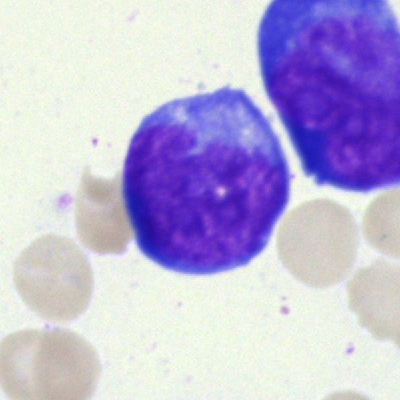
\includegraphics[width = \mywidth\textwidth]{pics/Anhang/single01}}
\quad
\subfloat[Referenz 2]{
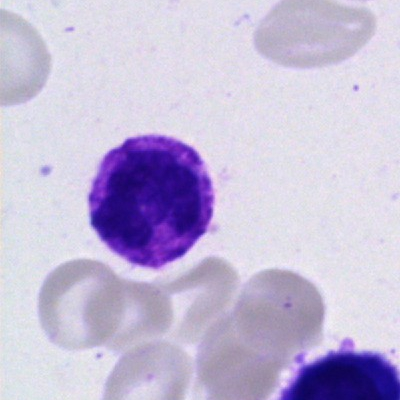
\includegraphics[width = \mywidth\textwidth]{pics/Anhang/single02}}
\quad
\subfloat[Referenz 3]{
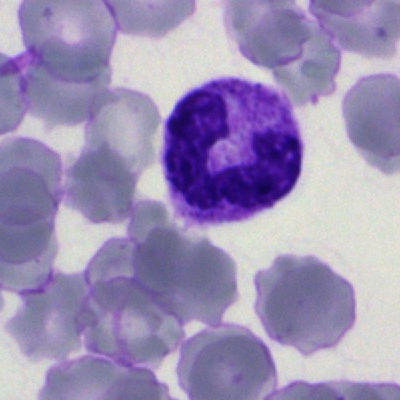
\includegraphics[width = \mywidth\textwidth]{pics/Anhang/single03}}
\quad
\subfloat[Referenz 4]{
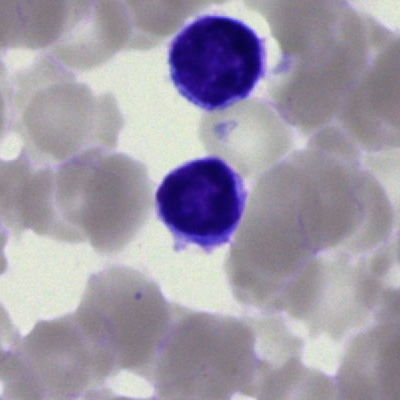
\includegraphics[width = \mywidth\textwidth]{pics/Anhang/single04}}
\quad
\subfloat[Referenz 5]{
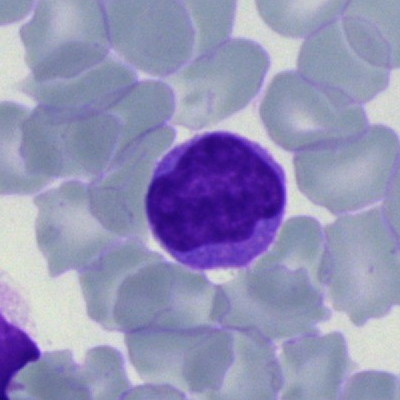
\includegraphics[width = \mywidth\textwidth]{pics/Anhang/single05}}
\quad
\subfloat[Referenz 6]{
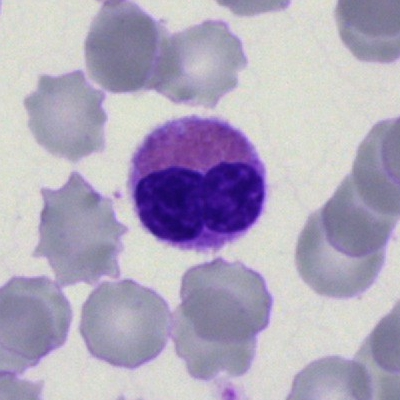
\includegraphics[width = \mywidth\textwidth]{pics/Anhang/single06}}
\quad
\subfloat[Referenz 7]{
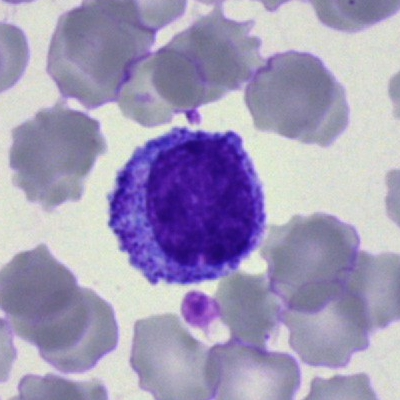
\includegraphics[width = \mywidth\textwidth]{pics/Anhang/single07}}
\quad
\subfloat[Referenz 8]{
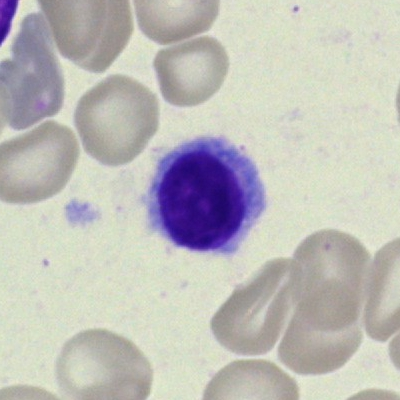
\includegraphics[width = \mywidth\textwidth]{pics/Anhang/single08}}
\quad
\subfloat[Referenz 9]{
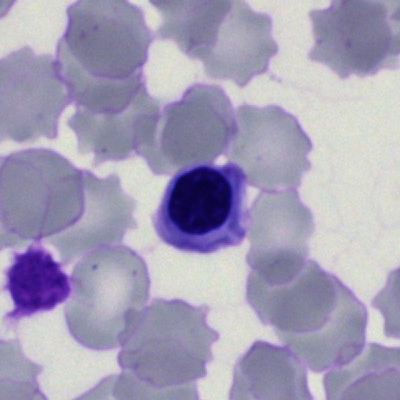
\includegraphics[width = \mywidth\textwidth]{pics/Anhang/single09}}
\quad
\subfloat[Referenz 10]{
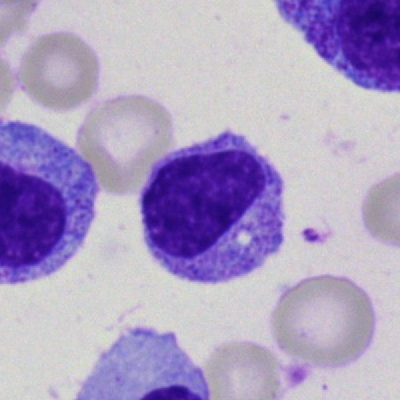
\includegraphics[width = \mywidth\textwidth]{pics/Anhang/single10}}
\quad
\subfloat[Referenz 11]{
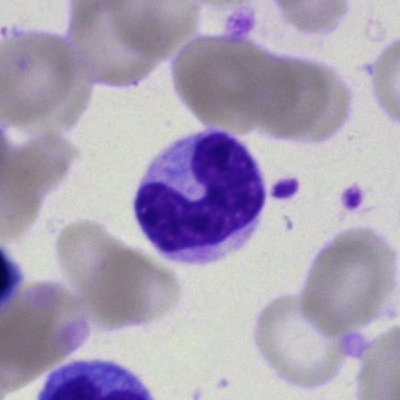
\includegraphics[width = \mywidth\textwidth]{pics/Anhang/single11}}
\quad
\subfloat[Referenz 12]{
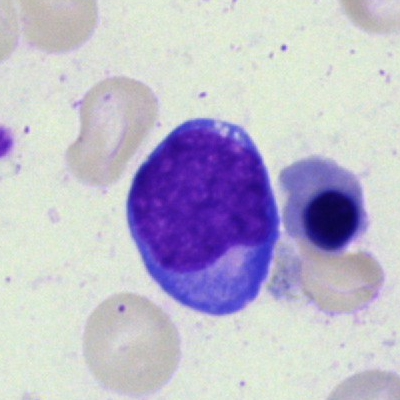
\includegraphics[width = \mywidth\textwidth]{pics/Anhang/single12}}
\quad
\subfloat[Referenz 13]{
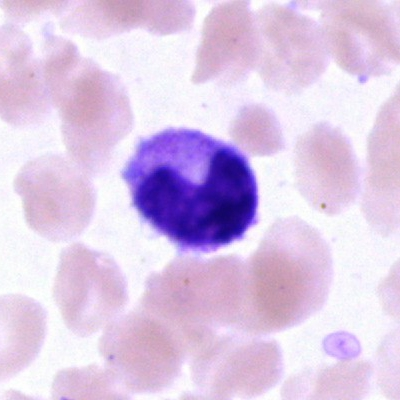
\includegraphics[width = \mywidth\textwidth]{pics/Anhang/single13}}
\quad
\subfloat[Referenz 14]{
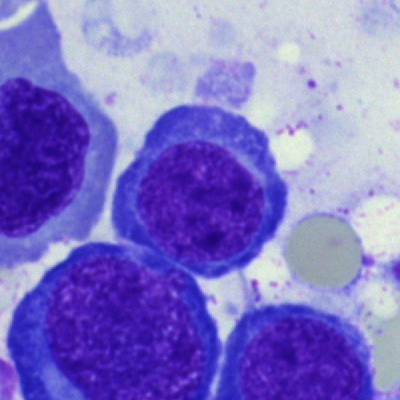
\includegraphics[width = \mywidth\textwidth]{pics/Anhang/single14}}
\quad
\subfloat[Referenz 15]{
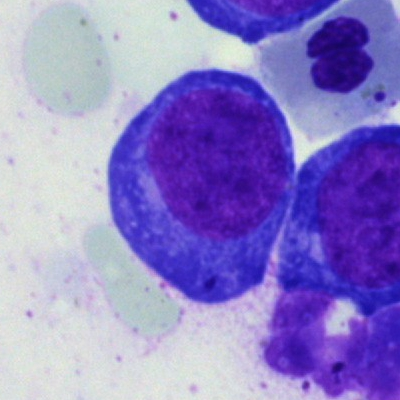
\includegraphics[width = \mywidth\textwidth]{pics/Anhang/single15}}
\caption{Alle Referenzbilder\label{fig:all_references}}
\end{figure}

\begin{table}[h!]
\center
\caption{Zusammensetzung Referenzsets}
\begin{tabular}{|c|r|}
\hline
\textbf{Set} & \textbf{Zusammensetzung} \\ 
\hline
3 & 1-15 \\ 
\hline 
4 & ohne 1,10,11,14\\ 
\hline 
5 & 2,5,6,8,9,15 \\ 
\hline 
6 & 2,8,9 \\ 
\hline
7 & 1,2,4,10,12,14,15\\
\hline
\end{tabular} 
\end{table}

\newpage

\refstepcounter{chapter}
\chaptermark{�berwicht Wirkung Normalisierungsmethoden}
\phantomsection
\addcontentsline{toc}{chapter}{\numberline{B}�bersicht Wirkung Normalisierungsmethoden}
\section{�bersicht Wirkung Normalisierungsmethoden}
\renewcommand{\mywidth}{0.17}
\begin{figure}[h]
\center
\subfloat{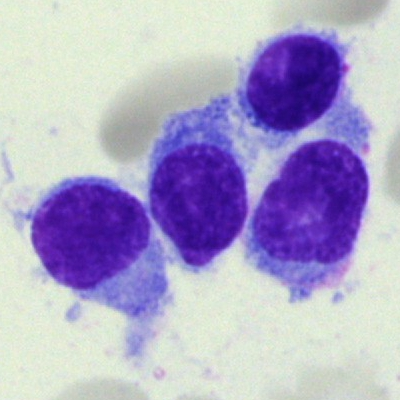
\includegraphics[width = \mywidth\textwidth]{pics/Anhang/B/01_or}}
\quad
\subfloat{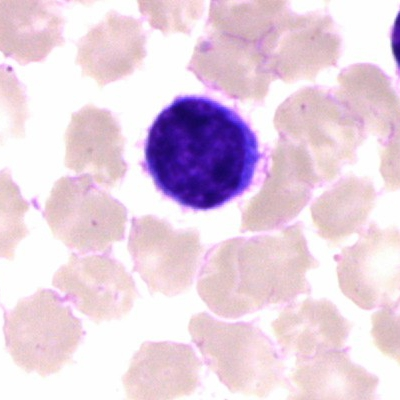
\includegraphics[width = \mywidth\textwidth]{pics/Anhang/B/02_or}}
\quad
\subfloat{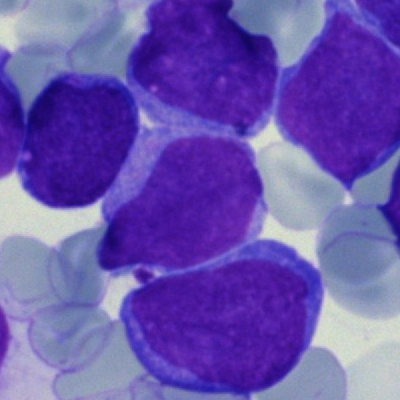
\includegraphics[width = \mywidth\textwidth]{pics/Anhang/B/03_or}}
\quad
\subfloat{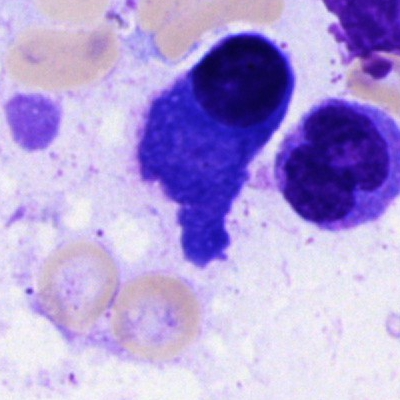
\includegraphics[width = \mywidth\textwidth]{pics/Anhang/B/04_or}}
\quad
\subfloat{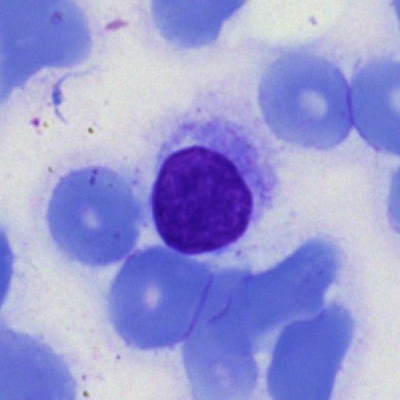
\includegraphics[width = \mywidth\textwidth]{pics/Anhang/B/05_or}}
\quad
\subfloat{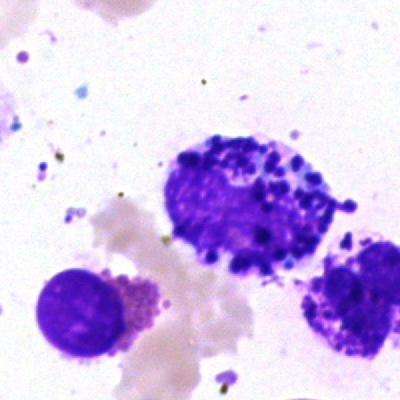
\includegraphics[width = \mywidth\textwidth]{pics/Anhang/B/06_or}}
\quad
\subfloat{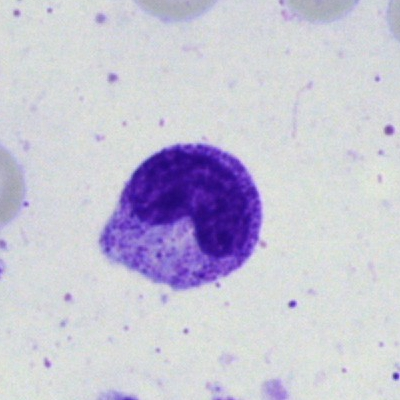
\includegraphics[width = \mywidth\textwidth]{pics/Anhang/B/07_or}}
\quad
\subfloat{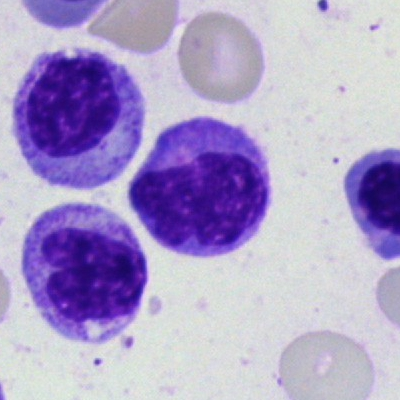
\includegraphics[width = \mywidth\textwidth]{pics/Anhang/B/08_or}}
\quad
\subfloat{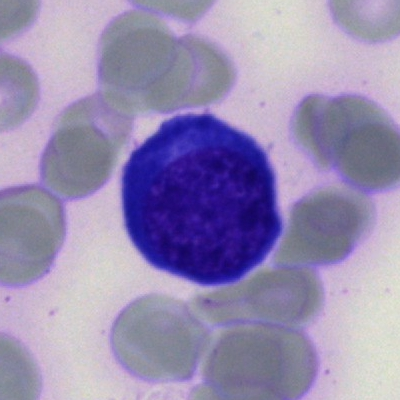
\includegraphics[width = \mywidth\textwidth]{pics/Anhang/B/09_or}}
\quad
\subfloat{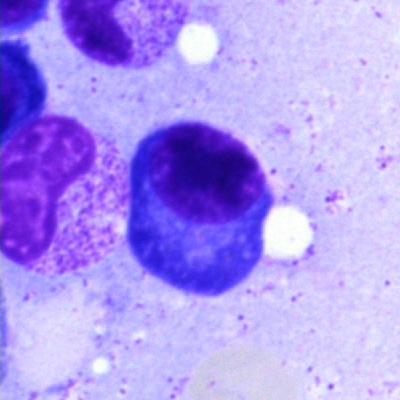
\includegraphics[width = \mywidth\textwidth]{pics/Anhang/B/10_or}}
\quad
\subfloat{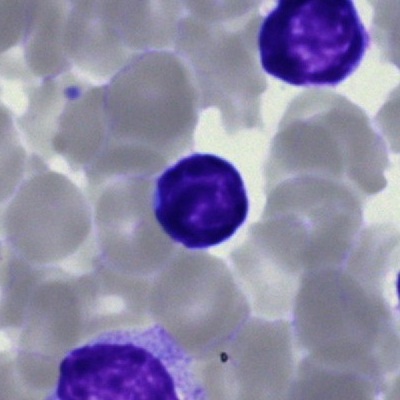
\includegraphics[width = \mywidth\textwidth]{pics/Anhang/B/11_or}}
\quad
\subfloat{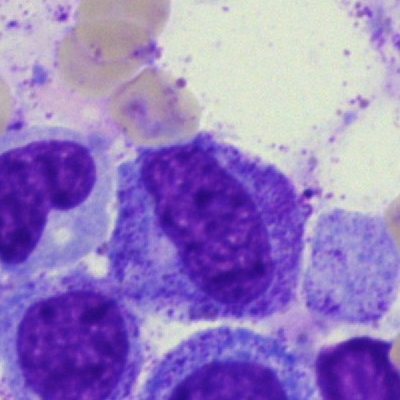
\includegraphics[width = \mywidth\textwidth]{pics/Anhang/B/12_or}}
\quad
\subfloat{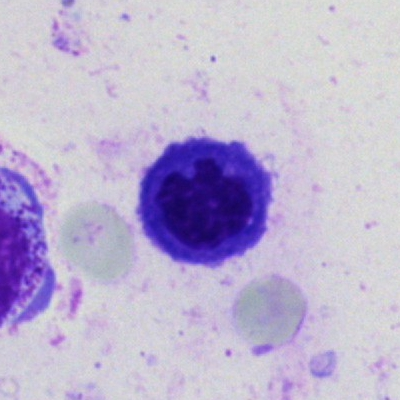
\includegraphics[width = \mywidth\textwidth]{pics/Anhang/B/13_or}}
\quad
\subfloat{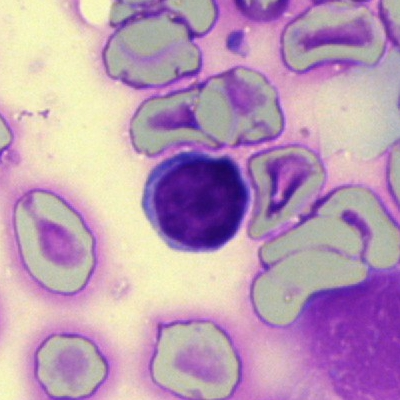
\includegraphics[width = \mywidth\textwidth]{pics/Anhang/B/14_or}}
\quad
\subfloat{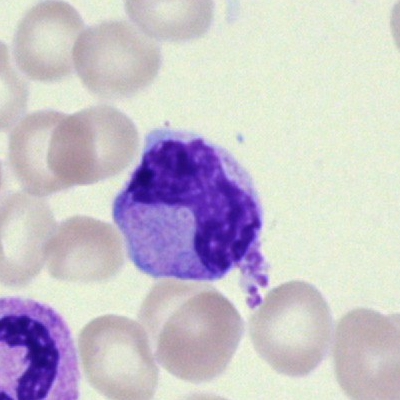
\includegraphics[width = \mywidth\textwidth]{pics/Anhang/B/15_or}}
\quad
\subfloat{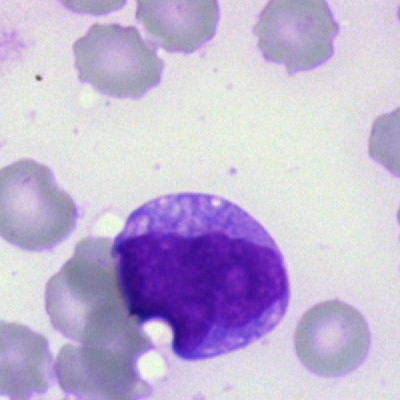
\includegraphics[width = \mywidth\textwidth]{pics/Anhang/B/16_or}}
\quad
\subfloat{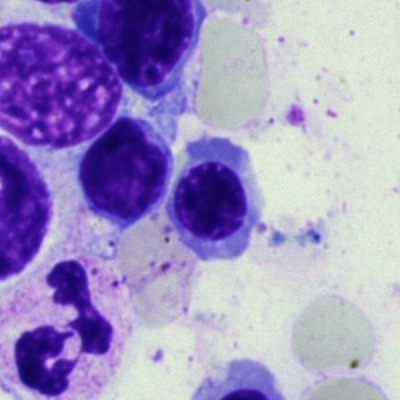
\includegraphics[width = \mywidth\textwidth]{pics/Anhang/B/17_or}}
\quad
\subfloat{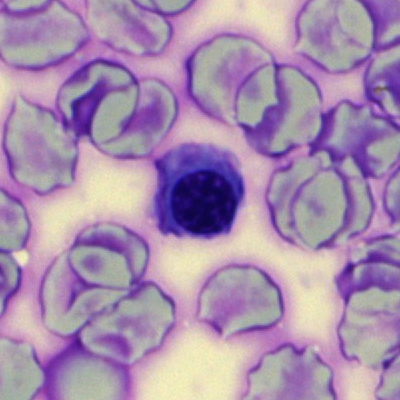
\includegraphics[width = \mywidth\textwidth]{pics/Anhang/B/18_or}}
\quad
\subfloat{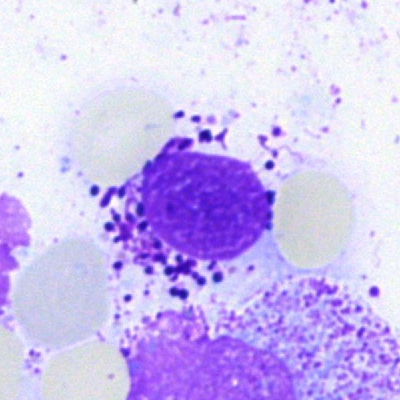
\includegraphics[width = \mywidth\textwidth]{pics/Anhang/B/19_or}}
\quad
\subfloat{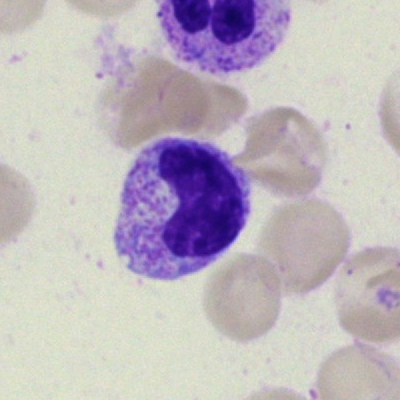
\includegraphics[width = \mywidth\textwidth]{pics/Anhang/B/20_or}}
\quad
\subfloat{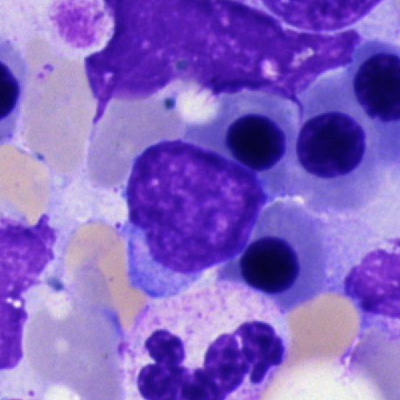
\includegraphics[width = \mywidth\textwidth]{pics/Anhang/B/21_or}}
\quad
\subfloat{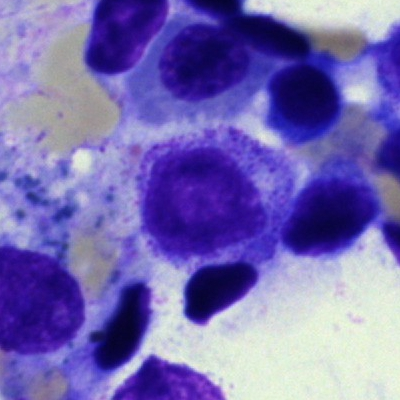
\includegraphics[width = \mywidth\textwidth]{pics/Anhang/B/22_or}}
\quad
\subfloat{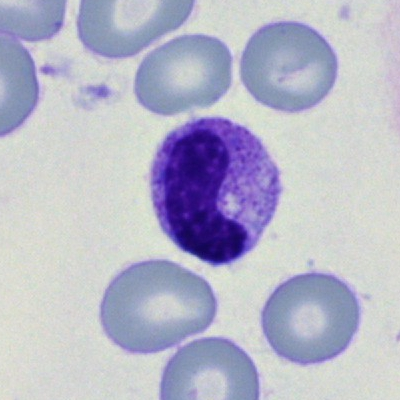
\includegraphics[width = \mywidth\textwidth]{pics/Anhang/B/23_or}}
\quad
\subfloat{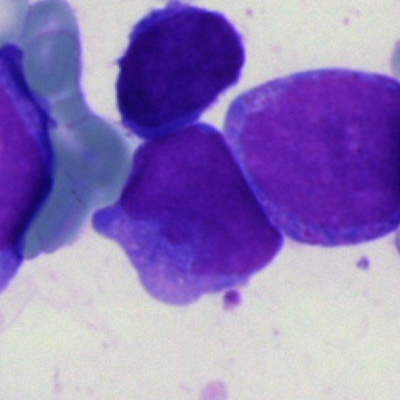
\includegraphics[width = \mywidth\textwidth]{pics/Anhang/B/24_or}}
\quad
\subfloat{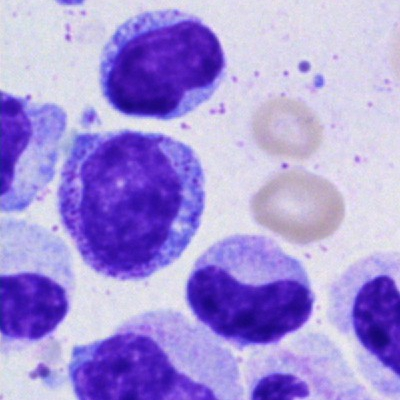
\includegraphics[width = \mywidth\textwidth]{pics/Anhang/B/25_or}}
\caption{Originalbilder\label{fig:25_original}}

\end{figure}
%Hier ein anderer Inhalt 
